\documentclass[11pt]{article}
\addtolength{\oddsidemargin}{-1.cm}
\addtolength{\textwidth}{2cm}
\addtolength{\topmargin}{-2cm}
\addtolength{\textheight}{3.5cm}

\usepackage[pdftex]{graphicx}
\usepackage{pdflscape}
\usepackage{hyperref}
\usepackage{float}
\usepackage{cite}
\usepackage{rotating}
\usepackage{graphicx}
\hypersetup{
	colorlinks=true,
	linkcolor=black,
	filecolor=magenta,
	urlcolor=cyan,
}

% define the title
\author{Team GladiOS Notification}
\title{Testing NavUP Longsword Notification Module}

\begin{document}
	\setlength{\parskip}{6pt}
	
	% generates the Cover page
	\begin{titlepage}
	\begin{center}
		% Upper part of the page       
		
\includegraphics[width=0.7\linewidth]{uniLogo.jpg}\\[1cm]
		
\includegraphics[width=0.7\linewidth]{headerCS.jpg}\\[1cm]  
		% Title
		\rule{\linewidth}{0.5mm} \\[1cm]
		{ \huge \bfseries  Testing Report \\\textbf{Team  CodeX}}\\[0.5cm]
		\rule{\linewidth}{0.5mm} \\[1cm] 			
		  
		  
		\begin{minipage}{0.4\textwidth}
			\begin{flushleft} \large
				 Burgers, Heinrich
			\end{flushleft}
		\end{minipage}
		\begin{minipage}{0.4\textwidth}
			\begin{flushright} \large
				\emph{} \\
				15059538
			\end{flushright}
		\end{minipage}
		
		
		\begin{minipage}{0.4\textwidth}
			\begin{flushleft} \large
				\emph{} \\
				Bondjobo, Jocelyn  
			\end{flushleft}
		\end{minipage}
		\begin{minipage}{0.4\textwidth}
			\begin{flushright} \large
				\emph{} \\
				13232852
			\end{flushright}
		\end{minipage}
		
	
		\begin{minipage}{0.4\textwidth}
			\begin{flushleft} \large
				\emph{} \\	
				Kirker, Tim	
			\end{flushleft}
		\end{minipage}
		\begin{minipage}{0.4\textwidth}
			\begin{flushright} \large
				\emph{} \\
				11152402	
			\end{flushright}
		\end{minipage}
		
		
		\begin{minipage}{0.4\textwidth}
			\begin{flushleft} \large
				\emph{} \\
				Hammond, Eunice
			\end{flushleft}
		\end{minipage}
		\begin{minipage}{0.4\textwidth}
			\begin{flushright} \large
				\emph{} \\
				13222563
			\end{flushright}
		\end{minipage}
		
		       
		\begin{minipage}{0.4\textwidth}
			\begin{flushleft} \large
				\emph{} \\
				Malangu, Daniel
			\end{flushleft}
		\end{minipage}
		\begin{minipage}{0.4\textwidth}
			\begin{flushright} \large
				\emph{} \\
				13315120
			\end{flushright}
		\end{minipage}
				
	\end{center}
\end{titlepage}
	
	\tableofcontents
	
	\newpage
	
	\section{Functional Requirements}
	\subsection{Core Functionality}
	\subsubsection{Email}
	The core functionality of the notification module is to send email notifications to users. To test the core functionality we used the tests outlined in Table 1.
	The two use cases tested was sending a single email and sending a batch of emails.
	
	Service Contracts:
	\begin{itemize}
      \item Email to single user. Score: 7.4
      \item Emails to all users. Score: 0
    \end{itemize}
	\subsection{Innovations}
	\subsubsection{SMS}
	The SMS interface has been declared but the functions are not implemented. This means that all the tests we ran failed due to their function returning a hard coded values. No SMS messages were received. The tests we used to test the SMS functionality is outlined in Table 2. The two use cases tested was sending a single SMS and sending a batch of SMS messages.
	
	Service Contracts:
	\begin{itemize}
      \item SMS message to single user. Score: 0
      \item SMS messages to all users. Score: 0
    \end{itemize}
	\subsubsection{Push Notifications}
	The Push Notification interface has been declared but the functions are not implemented. This means that all the test we ran failed due to their functions returning hard coded values. Though the interface cannot initialize a push notification the push notification sub-module is able to issue push notifications to user devices. This was verified by separate tests. The tests we ran on the interface is outlined in Table 3. The two use cases tested was sending a single push notification and sending a batch of push notifications.
	
	Service Contracts:
	\begin{itemize}
      \item Push Notification to single user. Score: 0
      \item Push Notifications to all users. Score: 0
    \end{itemize}
	
	\section{Non-Functional Requirements}
	Our tests for non-functional requirements can be found in Table 4. 
	
	\subsection{Performance}
    The email tests concluded that the system is able to send 100 emails in 8.02 minutes.
    The system is therefore inefficient in its real time processing as it unable to send batch emails and starts a new SMTP session for every email sent rather than opening up one session for all emails that need to be sent, which is a poor utilization of resources. The system is effective however, as it is able to send an email but ineffective when sending SMS messages or push notifications due to their interfaces not being implemented.
    
    We score their performance a 6.
    
    \subsection{Quality}
    The system is reliable in the sense that it is able to send 100 emails and all are delivered successfully. However it is unreliable in the sense that it is unable to send multiple emails in a timely manner as required. It also returns true when the SMS and push notifications are tested without them actually doing anything due to their interface functions not being implemnted. The system is almost always available as long as they have an internet connection and a valid email, we assume this because they use Google's Gmail SMTP service which has a 99.99\% uptime.
    
    We score their quality a 6.
    
    \subsection{Security}
    Data security is a very important aspect in any system. There is no exception in this module, any data sent by the module should be secure and only the party who the email is intended for should be able to view the content of the email. This module uses Google's Gmail SMTP service. The Gmail SMTP service requires a TLS (Transport Layer Security) session. This is acomplished with TTLS(Tunneled Transport Layer Security). TTLS is an EAP (Extensible Authentication Protocol) method that encapsulates a TLS session, consisting of a handshake phase and a data phase. This ensures that the data being sent between the notification module and Gmail's SMTP server is encrypted. This can be verified using WireShark to sniff the SMTP and TTL packets. A screen-shot of the packet sniff is on Figure 1. The line in blue shows that Gmail acknowledged the start of the TLS. Everything after this line will be encrypted. We could not verify this for SMS messages and push notifications because thier interfaces were not implemnted.
    
    We score their security a 10.
    
    \begin{figure}[h!]
      \caption{SMTP WireShark Trace}
      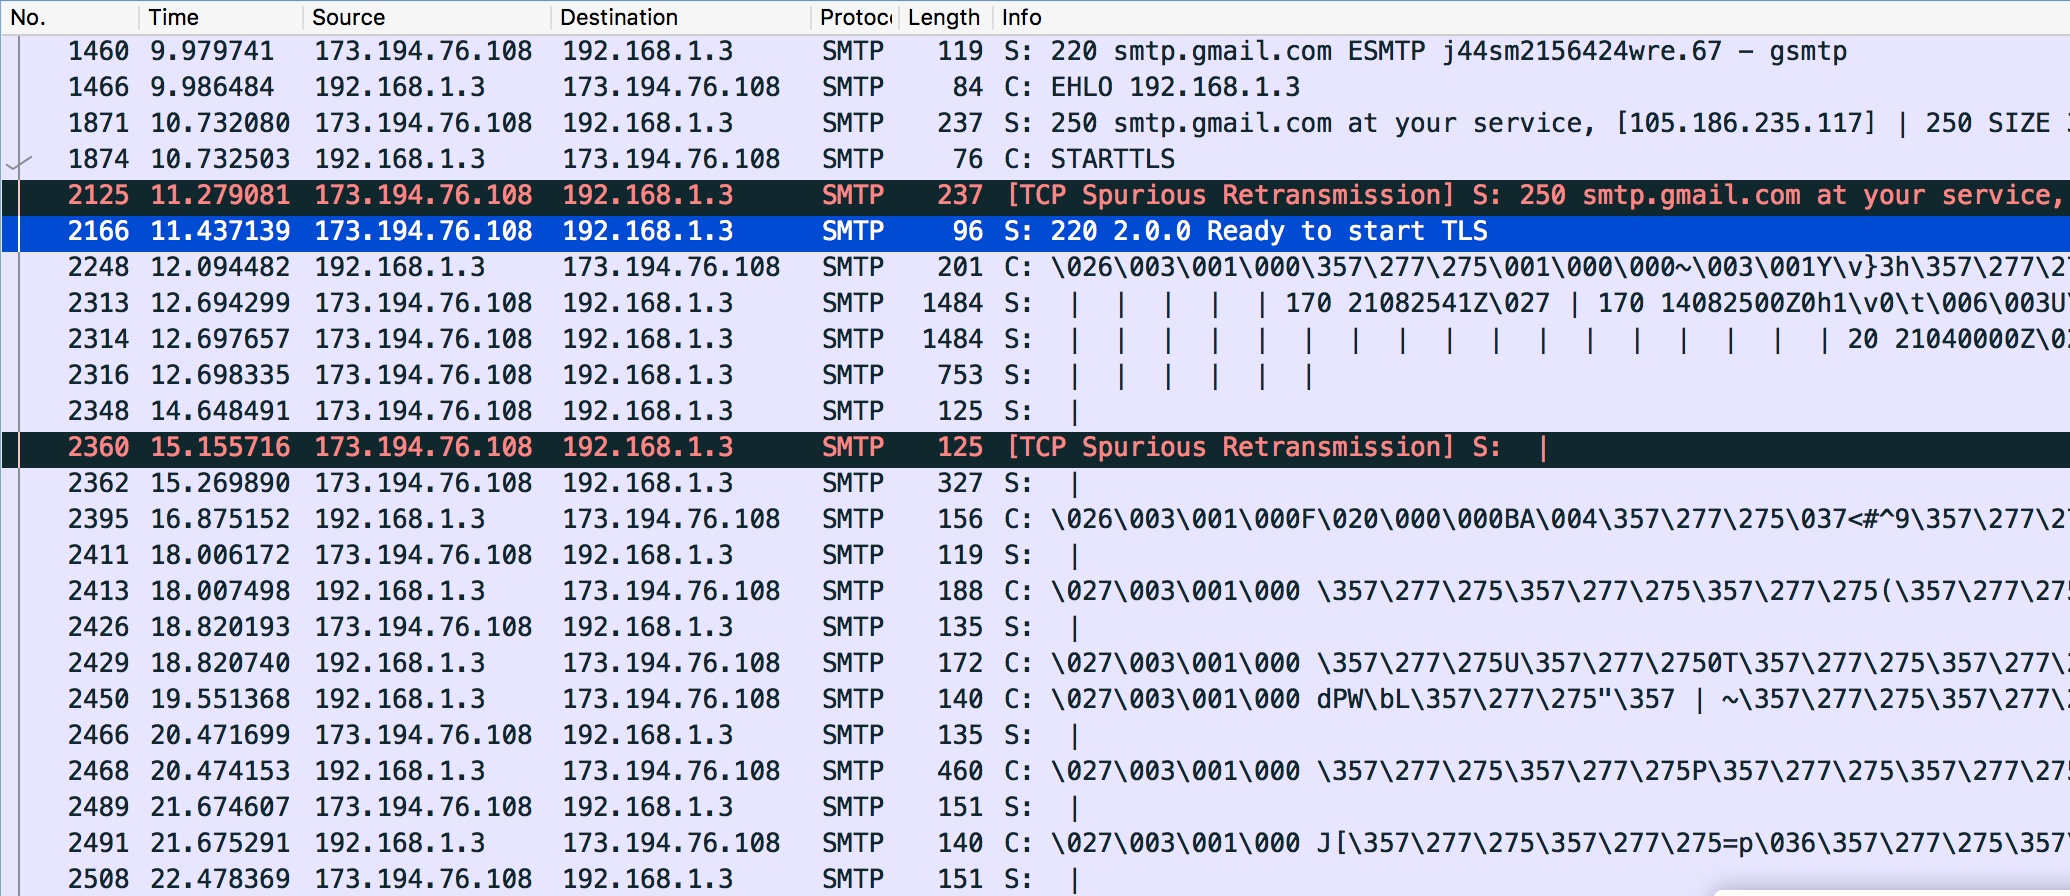
\includegraphics[width=\textwidth]{smtp.jpeg}
    \end{figure}
        
    \newpage
        
	\begin{sidewaystable}
        \centering
        \caption{My caption}
        \label{my-label}
        \begin{tabular}{lllllrr}
        \multicolumn{7}{c}{\textbf{Test Email to Single User}}                                                                                                                                                                                                                                                                                                                                                                                                                                                                                                                                                                                                                                                                                                                                         \\ \hline
        \multicolumn{1}{|l|}{Test}                                                                                                     & \multicolumn{1}{l|}{Input}                                                                                                                                                & \multicolumn{1}{l|}{Expected Result}                                                                       & \multicolumn{1}{l|}{Actual Result}                                                                         & \multicolumn{1}{l|}{Comment}                                                                                                                                                                 & \multicolumn{1}{l|}{Score} & \multicolumn{1}{l|}{Weight} \\ \hline
        \multicolumn{1}{|l|}{\begin{tabular}[c]{@{}l@{}}Send single \\ email to user.\end{tabular}}                                    & \multicolumn{1}{l|}{\begin{tabular}[c]{@{}l@{}}Email: u15029779@\\ tuks.co.za\\ Subject: Longsword\\ Notification\\ Message: Longsword\\ notification test.\end{tabular}} & \multicolumn{1}{l|}{\begin{tabular}[c]{@{}l@{}}\{'success':'true',\\ 'Error':'None'\}\end{tabular}}        & \multicolumn{1}{l|}{\begin{tabular}[c]{@{}l@{}}\{'success':'true',\\ 'Error':'None'\}\end{tabular}}        & \multicolumn{1}{l|}{}                                                                                                                                                                        & \multicolumn{1}{r|}{10}    & \multicolumn{1}{r|}{0.5}    \\ \hline
        \multicolumn{1}{|l|}{\begin{tabular}[c]{@{}l@{}}Send single \\ email to user \\ with a empty \\ message.\end{tabular}}         & \multicolumn{1}{l|}{\begin{tabular}[c]{@{}l@{}}Email: u15029779@\\ tuks.co.za\\ Subject: Longsword\\ Notification\\ Message:\end{tabular}}                                & \multicolumn{1}{l|}{\begin{tabular}[c]{@{}l@{}}\{'success':'false',\\ 'Error':'some error'\}\end{tabular}} & \multicolumn{1}{l|}{\begin{tabular}[c]{@{}l@{}}\{'success':'true', \\ 'Error':'none'\}\end{tabular}}       & \multicolumn{1}{l|}{\begin{tabular}[c]{@{}l@{}}The email is still sent and the \\ function returns true.\end{tabular}}                                                                       & \multicolumn{1}{r|}{0}     & \multicolumn{1}{r|}{0.2}    \\ \hline
        \multicolumn{1}{|l|}{\begin{tabular}[c]{@{}l@{}}Send single \\ email to user \\ with a invalid \\ email address.\end{tabular}} & \multicolumn{1}{l|}{\begin{tabular}[c]{@{}l@{}}Email: u15029779\\ Subject: Longsword \\ Notification\\ Message: Longsword\\ notification test.\end{tabular}}              & \multicolumn{1}{l|}{\begin{tabular}[c]{@{}l@{}}\{'success':'false',\\ 'Error':'some error'\}\end{tabular}} & \multicolumn{1}{l|}{\begin{tabular}[c]{@{}l@{}}\{'success':'true', \\ 'Error':'some error'\}\end{tabular}} & \multicolumn{1}{l|}{\begin{tabular}[c]{@{}l@{}}Their function returns true \\ when an error occurs, but \\ does provide the error \\ description and the email \\ is not sent.\end{tabular}} & \multicolumn{1}{r|}{8}     & \multicolumn{1}{r|}{0.3}    \\ \hline
                                                                                                                                       &                                                                                                                                                                           &                                                                                                            & \multicolumn{1}{l|}{}                                                                                      & \multicolumn{1}{l|}{Total}                                                                                                                                                                   & \multicolumn{2}{r|}{7.4}                                 \\ \cline{5-7} 
                                                                                                                                       &                                                                                                                                                                           &                                                                                                            &                                                                                                            &                                                                                                                                                                                              & \multicolumn{1}{l}{}       & \multicolumn{1}{l}{}        \\
        \multicolumn{7}{c}{\textbf{Test Emails To All}}                                                                                                                                                                                                                                                                                                                                                                                                                                                                                                                                                                                                                                                                                                                                                \\ \hline
        \multicolumn{1}{|l|}{Test}                                                                                                     & \multicolumn{1}{l|}{Input}                                                                                                                                                & \multicolumn{1}{l|}{Expected Result}                                                                       & \multicolumn{1}{l|}{Actual Result}                                                                         & \multicolumn{1}{l|}{Comment}                                                                                                                                                                 & \multicolumn{1}{l|}{Score} & \multicolumn{1}{l|}{Weight} \\ \hline
        \multicolumn{1}{|l|}{\begin{tabular}[c]{@{}l@{}}Send email to \\ all users.\end{tabular}}                                      & \multicolumn{1}{l|}{\begin{tabular}[c]{@{}l@{}}Message: Testing Email\\ to All\end{tabular}}                                                                              & \multicolumn{1}{l|}{\begin{tabular}[c]{@{}l@{}}\{'success':'true',\\ 'Error':'None'\}\end{tabular}}        & \multicolumn{1}{l|}{Empty String}                                                                          & \multicolumn{1}{l|}{\begin{tabular}[c]{@{}l@{}}Their function is empty\\ and returns empty string.\end{tabular}}                                                                             & \multicolumn{1}{r|}{0}     & \multicolumn{1}{r|}{0.5}    \\ \hline
        \multicolumn{1}{|l|}{\begin{tabular}[c]{@{}l@{}}Send single \\ email to user \\ with a empty \\ message.\end{tabular}}         & \multicolumn{1}{l|}{Message:}                                                                                                                                             & \multicolumn{1}{l|}{\begin{tabular}[c]{@{}l@{}}\{'success':'false',\\ 'Error':'some error'\}\end{tabular}} & \multicolumn{1}{l|}{Empty String}                                                                          & \multicolumn{1}{l|}{\begin{tabular}[c]{@{}l@{}}Their function is empty \\ and returns empty string.\end{tabular}}                                                                            & \multicolumn{1}{r|}{0}     & \multicolumn{1}{r|}{0.2}    \\ \hline
                                                                                                                                       &                                                                                                                                                                           &                                                                                                            & \multicolumn{1}{l|}{}                                                                                      & \multicolumn{1}{l|}{Total}                                                                                                                                                                   & \multicolumn{2}{r|}{0}                                   \\ \cline{5-7} 
        \end{tabular}
    \end{sidewaystable}
    
    \begin{sidewaystable}
        \centering
        \caption{Test SMS}
        \label{my-label}
        \begin{tabular}{lllllrr}
        \multicolumn{7}{c}{\textbf{Test SMS to Single User}}                                                                                                                                                                                                                                                                                                                                                                                                                                                                                      \\ \hline
        \multicolumn{1}{|l|}{Test}                                                                                           & \multicolumn{1}{l|}{Input}                                                                                             & \multicolumn{1}{l|}{Expected Result} & \multicolumn{1}{l|}{Actual Result} & \multicolumn{1}{l|}{Comment}                                                                                                                       & \multicolumn{1}{l|}{Score} & \multicolumn{1}{l|}{Weight} \\ \hline
        \multicolumn{1}{|l|}{\begin{tabular}[c]{@{}l@{}}Send single \\ SMS to user.\end{tabular}}                            & \multicolumn{1}{l|}{\begin{tabular}[c]{@{}l@{}}User: User List\\ Message: SMS Test\end{tabular}}                       & \multicolumn{1}{l|}{true}            & \multicolumn{1}{l|}{true}          & \multicolumn{1}{l|}{\begin{tabular}[c]{@{}l@{}}Result is hard coded. \\ Function is not \\ implemented and SMS is \\ never received.\end{tabular}} & \multicolumn{1}{r|}{0}     & \multicolumn{1}{r|}{0.5}    \\ \hline
        \multicolumn{1}{|l|}{\begin{tabular}[c]{@{}l@{}}Send single \\ SMS to user \\ with a empty \\ message.\end{tabular}} & \multicolumn{1}{l|}{\begin{tabular}[c]{@{}l@{}}Users: User List\\ Message:\end{tabular}}                               & \multicolumn{1}{l|}{false}           & \multicolumn{1}{l|}{true}          & \multicolumn{1}{l|}{\begin{tabular}[c]{@{}l@{}}Result is hard coded. \\ Function is not \\ implemented.\end{tabular}}                              & \multicolumn{1}{r|}{0}     & \multicolumn{1}{r|}{0.2}    \\ \hline
        \multicolumn{1}{|l|}{\begin{tabular}[c]{@{}l@{}}Send single \\ SMS to user \\ with a invalid \\ user.\end{tabular}}  & \multicolumn{1}{l|}{\begin{tabular}[c]{@{}l@{}}User: User List\\ with invalid user.\\ Message: SMS  Test\end{tabular}} & \multicolumn{1}{l|}{false}           & \multicolumn{1}{l|}{true}          & \multicolumn{1}{l|}{\begin{tabular}[c]{@{}l@{}}Result is hard coded. \\ Function is not \\ implemented.\end{tabular}}                              & \multicolumn{1}{r|}{0}     & \multicolumn{1}{r|}{0.3}    \\ \hline
                                                                                                                             &                                                                                                                        &                                      & \multicolumn{1}{l|}{}              & \multicolumn{1}{l|}{Total}                                                                                                                         & \multicolumn{2}{r|}{0}                                   \\ \cline{5-7} 
                                                                                                                             &                                                                                                                        &                                      &                                    &                                                                                                                                                    & \multicolumn{1}{l}{}       & \multicolumn{1}{l}{}        \\
        \multicolumn{7}{c}{\textbf{Test SMS To All}}                                                                                                                                                                                                                                                                                                                                                                                                                                                                                              \\ \hline
        \multicolumn{1}{|l|}{Test}                                                                                           & \multicolumn{1}{l|}{Input}                                                                                             & \multicolumn{1}{l|}{Expected Result} & \multicolumn{1}{l|}{Actual Result} & \multicolumn{1}{l|}{Comment}                                                                                                                       & \multicolumn{1}{l|}{Score} & \multicolumn{1}{l|}{Weight} \\ \hline
        \multicolumn{1}{|l|}{\begin{tabular}[c]{@{}l@{}}Send SMS to \\ all users.\end{tabular}}                              & \multicolumn{1}{l|}{\begin{tabular}[c]{@{}l@{}}Message: Testing SMS\\ to all\end{tabular}}                             & \multicolumn{1}{l|}{true}            & \multicolumn{1}{l|}{true}          & \multicolumn{1}{l|}{\begin{tabular}[c]{@{}l@{}}Result is hard coded. \\ Function is not \\ implemented and SMS is \\ never received.\end{tabular}} & \multicolumn{1}{r|}{0}     & \multicolumn{1}{r|}{0.5}    \\ \hline
        \multicolumn{1}{|l|}{\begin{tabular}[c]{@{}l@{}}Send SMS to\\ all users with \\ a empty \\ message.\end{tabular}}    & \multicolumn{1}{l|}{Message:}                                                                                          & \multicolumn{1}{l|}{false}           & \multicolumn{1}{l|}{true}          & \multicolumn{1}{l|}{\begin{tabular}[c]{@{}l@{}}Result is hard coded. \\ Function is not \\ implemented.\end{tabular}}                              & \multicolumn{1}{r|}{0}     & \multicolumn{1}{r|}{0.2}    \\ \hline
                                                                                                                             &                                                                                                                        &                                      & \multicolumn{1}{l|}{}              & \multicolumn{1}{l|}{Total}                                                                                                                         & \multicolumn{2}{r|}{0}                                   \\ \cline{5-7} 
        \end{tabular}
    \end{sidewaystable}
    
    \begin{sidewaystable}
        \centering
        \caption{Test Push Notification}
        \label{my-label}
        \begin{tabular}{lllllrr}
        \multicolumn{7}{c}{\textbf{Test Push Notification to Single User}}                                                                                                                                                                                                                                                                                                                                                                                                                                                                                                                            \\ \hline
        \multicolumn{1}{|l|}{Test}                                                                                                         & \multicolumn{1}{l|}{Input}                                                                                              & \multicolumn{1}{l|}{Expected Result} & \multicolumn{1}{l|}{Actual Result} & \multicolumn{1}{l|}{Comment}                                                                                                                                                            & \multicolumn{1}{l|}{Score} & \multicolumn{1}{l|}{Weight} \\ \hline
        \multicolumn{1}{|l|}{\begin{tabular}[c]{@{}l@{}}Send single \\ Push Notification\\ to user.\end{tabular}}                          & \multicolumn{1}{l|}{\begin{tabular}[c]{@{}l@{}}User: User List\\ Message: Push Test\end{tabular}}                       & \multicolumn{1}{l|}{true}            & \multicolumn{1}{l|}{true}          & \multicolumn{1}{l|}{\begin{tabular}[c]{@{}l@{}}Result is hard coded. \\ Function is not \\ implemented and Push \\ Notification is never \\ initiated from the interface.\end{tabular}} & \multicolumn{1}{r|}{0}     & \multicolumn{1}{r|}{0.5}    \\ \hline
        \multicolumn{1}{|l|}{\begin{tabular}[c]{@{}l@{}}Send single \\ Push Notification \\ to user with a\\ empty message.\end{tabular}}  & \multicolumn{1}{l|}{\begin{tabular}[c]{@{}l@{}}Users: User List\\ Message:\end{tabular}}                                & \multicolumn{1}{l|}{false}           & \multicolumn{1}{l|}{true}          & \multicolumn{1}{l|}{\begin{tabular}[c]{@{}l@{}}Result is hard coded. \\ Function is not \\ implemented.\end{tabular}}                                                                   & \multicolumn{1}{r|}{0}     & \multicolumn{1}{r|}{0.2}    \\ \hline
        \multicolumn{1}{|l|}{\begin{tabular}[c]{@{}l@{}}Send single \\ Push Notification\\ to user with a \\ invalid user.\end{tabular}}   & \multicolumn{1}{l|}{\begin{tabular}[c]{@{}l@{}}User: User List\\ with invalid user.\\ Message: Push  Test\end{tabular}} & \multicolumn{1}{l|}{false}           & \multicolumn{1}{l|}{true}          & \multicolumn{1}{l|}{\begin{tabular}[c]{@{}l@{}}Result is hard coded. \\ Function is not \\ implemented.\end{tabular}}                                                                   & \multicolumn{1}{r|}{0}     & \multicolumn{1}{r|}{0.3}    \\ \hline
                                                                                                                                           &                                                                                                                         &                                      & \multicolumn{1}{l|}{}              & \multicolumn{1}{l|}{Total}                                                                                                                                                              & \multicolumn{2}{r|}{0}                                   \\ \cline{5-7} 
                                                                                                                                           &                                                                                                                         &                                      &                                    &                                                                                                                                                                                         & \multicolumn{1}{l}{}       & \multicolumn{1}{l}{}        \\
        \multicolumn{7}{c}{\textbf{Test Push Notification To All}}                                                                                                                                                                                                                                                                                                                                                                                                                                                                                                                                    \\ \hline
        \multicolumn{1}{|l|}{Test}                                                                                                         & \multicolumn{1}{l|}{Input}                                                                                              & \multicolumn{1}{l|}{Expected Result} & \multicolumn{1}{l|}{Actual Result} & \multicolumn{1}{l|}{Comment}                                                                                                                                                            & \multicolumn{1}{l|}{Score} & \multicolumn{1}{l|}{Weight} \\ \hline
        \multicolumn{1}{|l|}{\begin{tabular}[c]{@{}l@{}}Send Push \\ Notification to \\ all users.\end{tabular}}                           & \multicolumn{1}{l|}{\begin{tabular}[c]{@{}l@{}}Message: Testing Push\\ to all\end{tabular}}                             & \multicolumn{1}{l|}{true}            & \multicolumn{1}{l|}{true}          & \multicolumn{1}{l|}{\begin{tabular}[c]{@{}l@{}}Result is hard coded. \\ Function is not \\ implemented and Push \\ Notification is never \\ initiated from the interface.\end{tabular}} & \multicolumn{1}{r|}{0}     & \multicolumn{1}{r|}{0.5}    \\ \hline
        \multicolumn{1}{|l|}{\begin{tabular}[c]{@{}l@{}}Send Push \\ Notification to\\ all users with \\ a empty \\ message.\end{tabular}} & \multicolumn{1}{l|}{Message:}                                                                                           & \multicolumn{1}{l|}{false}           & \multicolumn{1}{l|}{true}          & \multicolumn{1}{l|}{\begin{tabular}[c]{@{}l@{}}Result is hard coded. \\ Function is not \\ implemented.\end{tabular}}                                                                   & \multicolumn{1}{r|}{0}     & \multicolumn{1}{r|}{0.2}    \\ \hline
                                                                                                                                           &                                                                                                                         &                                      & \multicolumn{1}{l|}{}              & \multicolumn{1}{l|}{Total}                                                                                                                                                              & \multicolumn{2}{r|}{0}                                   \\ \cline{5-7} 
        \end{tabular}
	\end{sidewaystable}
	
	\begin{sidewaystable}
	    \centering
        \caption{Non-Functonal Requirements Tests}
        \label{my-label}
        \begin{tabular}{lllll}
        \multicolumn{5}{c}{\textbf{Test Performance}}                                                                                                                                                                                                                                                                                                                                                                                                                                                                                                                                           \\ \hline
        \multicolumn{1}{|l|}{Test}            & \multicolumn{1}{l|}{Input}                                                                                                                                                & \multicolumn{1}{l|}{Expected Result}                                                                & \multicolumn{1}{l|}{Actual Result}                                                                   & \multicolumn{1}{l|}{Comment}                                                                                                                           \\ \hline
        \multicolumn{1}{|l|}{Send 50 Emails}  & \multicolumn{1}{l|}{\begin{tabular}[c]{@{}l@{}}Email: u15029779@\\ tuks.co.za\\ Subject: Longsword\\ Notification\\ Message: Longsword\\ notification test.\end{tabular}} & \multicolumn{1}{l|}{\begin{tabular}[c]{@{}l@{}}\{'success':'true',\\ 'Error':'None'\}\end{tabular}} & \multicolumn{1}{l|}{\begin{tabular}[c]{@{}l@{}}\{'success':'true',\\ 'Error':'None'\}\end{tabular}}  & \multicolumn{1}{l|}{\begin{tabular}[c]{@{}l@{}}All 50 emails are successfully sent.\\ They were all sent in 4 minutes and \\ 11 seconds\end{tabular}}  \\ \hline
        \multicolumn{1}{|l|}{Send 100 Emails} & \multicolumn{1}{l|}{\begin{tabular}[c]{@{}l@{}}Email: u15029779@\\ tuks.co.za\\ Subject: Longsword\\ Notification\\ Message:Longsword \\ notification test.\end{tabular}} & \multicolumn{1}{l|}{\begin{tabular}[c]{@{}l@{}}\{'success':'true',\\ 'Error':'none'\}\end{tabular}} & \multicolumn{1}{l|}{\begin{tabular}[c]{@{}l@{}}\{'success':'true', \\ 'Error':'none'\}\end{tabular}} & \multicolumn{1}{l|}{\begin{tabular}[c]{@{}l@{}}All 100 emails are successfully sent. \\ They were all sent in 8 minutes and \\ 2 seconds\end{tabular}} \\ \hline
        \end{tabular}
	\end{sidewaystable}
	
\end{document}
